\section{Datawarehouse}
	\noindent
	This section will provide an introductory overview over the datawarehousing discipline and commonly terminology within. 
	For the non-database gurus the datawarehousing dicispline is, for all intent and purposes, an organization schema of
	data created to enable and facilitate data analyses without the absolute focus on normalization. \cite{oracle:dataware}
	%Though not the only key features that differentiate datawarehouses from ordinary databases.
	%\cite{wiki:normalization, wiki:datawarehouse}
	
	\bigskip\noindent
	In the datawarehouse field you will often find buzz words describing commonly known principles from ordinary database
	usage. Some of the most used include \textit{facts table}, \textit{measures} and \textit{dimensions}.
	These words describe to a large extends the concepts around designing a datawarehouse. 
	
	\bigskip\noindent
	Measures are exactly what the avid reader may intuitively allready know, quantitative data about a business.
	While dimensions can be considered to be meta-data, and works as descriptive attributes. 
	As an example from the service industry, one can consider a storechain and each stores sales. 
	In this case one could look at each sale as a fact with price as possible \textit{measure},
	and store location as a \textit{dimension}. 
	The difference between measures and dimensions become more apparent when considering their usage.
	One common queryform would be to use an arithmetic function, as \texttt{average} or \texttt{sum}, over a set of
	\textit{measures} filtered by a value from the \textit{dimensional} set.
	The \textit{facts table} is the combination of these two, and hence holding all the "`facts"' related to 
	
	
	\bigskip\noindent
	In the further discussion of datawarehouses we will look at two prominent organizational schemas utilizes 
	within the datawarehouse discipline, namely star schema and snowflake schema. 
	Both of which have gotten their names by their resemblance to their respective natural phenomena.
	Common for the both of them is that the facts table serves as the main storage table in the schema, 
	and is often pictured as the center of the warehouse in graphical illustrations (see figures~\ref{fig:starSchemeConcept} and \ref{fig:snowflakeSchemeConcept}). 
	
	\bigskip\noindent
	Since the star schema is the simplest, and considered a special case of the snowflake schema
	we will start off with explaining the basics around this schema (See figure~\ref{fig:starSchemeConcept}). 
	The \textit{star schema} figure has the \textit{fact table} at its center, with the \textit{dimensional tables} at its peripheral. 
	These dimensional table are not normalized, and may contain duplicate entries, e.g. the \textit{date} of the entry.
		
	\begin{figure}[H]%
		\centering
		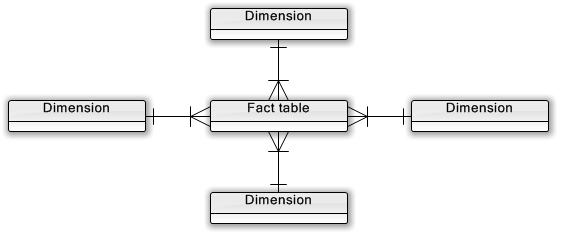
\includegraphics[width=0.5\columnwidth]{UML/StarSchemaConcept.png}%
		\caption{Star schema concept}%
		\label{fig:starSchemeConcept}%
	\end{figure}
	
	\bigskip\noindent
	The \textit{snowflake schema} show the same general structure as the \textit{star schema}, 
	but shows a difference in the way \textit{dimensions} are represented. 
	In the snowflake schema the \textit{dimensional tables} are more normalized, hence giving it the apparent snowflake look.
	Continuing with the \textit{date}	example from the the star schema explanation you'll note that dates has several natural 
	parts, e.g. year, month, day, hour ect. And hence can be normalized into these respective tables, 
	it is however more normal to augment the date with data consider with quarter in the year it belongs to. 
	Hence making it easy to aggregate data over each quarter instead of aggregating over several month.
	
	\begin{figure}[H]%
		\centering
		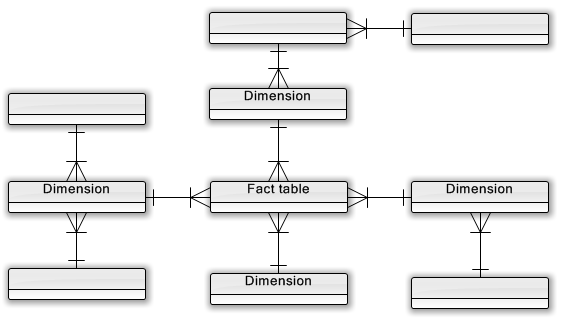
\includegraphics[width=0.5\columnwidth]{UML/SnowflakeSchemaConcept.png}%
		\caption{Star schema concept}%
		\label{fig:snowflakeSchemeConcept}%
	\end{figure}	
	
	\subsection{ETL workflow}
		The typical workflow when working with datawarehouses is \textit{extract, transform, load} or ETL. 
		The concrete implementation found in different datawarehouses may have considerable differences between them, 
		we will therefore not go into the implementations details at this point. But rather explain the basic concepts
		and motivation behind each step.
		
		\subsubsection{Extract}
			
		\subsubsection{Transform}
			
		\subsubsection{Load}
			